\section{Auswertung}
\label{sec:Auswertung}
\subsection{Vermessung von Spektrallinien}
\label{subsec:a0}
Es besteht die Möglichkeit allein durch Abzählen der Kanäle und der entsprechenden Zählergebnisse die Höhe, die Lage und den Inhalt einer Spektrallinie anzugeben.
Die Ergebnisse dieser Methode können jedoch nicht immer eindeutig angegeben werden, sodass eine unabhängige Auswertung unmöglich wird.
Hier wird daher eine andere Methode gewählt.
Zunächst wird die Lage einer Spektrallinie, wie oben auch, auf den Kanal mit dem höchsten Zählergebnis in einer hinreichend großen Umgebung geschätzt.
Um den so abgelesenen Kanal herum wird über die jeweils 20 oberhalb und unterhalb liegenden Kanäle eine Gauß-Funktion
\begin{align}
g(k)=c_1\exp\left(-c_2(k-c_3)^2\right)+c_4
\end{align}
an die Messdaten gefittet.
Dabei entspricht $c_1$ der Höhe der Spektrallinie und $c_3$ ihrer Lage.
Hier ist sofort ein Vorteil dieser Methode zu erkennen, denn die Lage einer Spektrallinie kann nun präziser als die Auflösung der Kanalskala angegeben werden.
Die Formel
\begin{align}
  \label{eqn:inhalt}
  \int_\infty^\infty c_1\exp\left(-c_2(k-c_3)^2\right) dk = c_1 \sqrt{\frac{\pi}{c_2}}
\end{align}
zeigt, dass $c_1$ und $c_2$ zusammen ein Maß für den Inhalt einer Spektrallinie sind.
Der Parameter $c_4$ dient dazu Störeffekte wie das Compton-Kontinuum oder die Untergrundstrahlung aus den folgenden Rechnungen zu eliminieren.
Er wird deshalb im Folgenden nicht weiter berücksichtigt.
Diese und jede weitere Regressionsrechnung in dieser Auswertung wird mithilfe der Funktion \textit{curve\_ fit} aus dem Python Paket \textit{scipy.optimize} durchgeführt.
Fehlerrechnungen werden ebenfalls von Python übernommen.
Dazu wird das Paket \textit{uncertainties} verwendet.

\subsection{Kallibration und Bestimmung der Effizienz}
\label{subsec:a1}
Um das Energiespektrum für unbekannte Strahler sinnvoll interpretieren zu können,
ist eine Kalibrierung der Energieskala notwendig. Dazu wird das linienreiche Spektrum eines Europium 152 Strahlers betrachtet, welches in Abbildung \ref{fig:spektrum_eu} dargestellt ist.
\begin{figure}
 \centering
 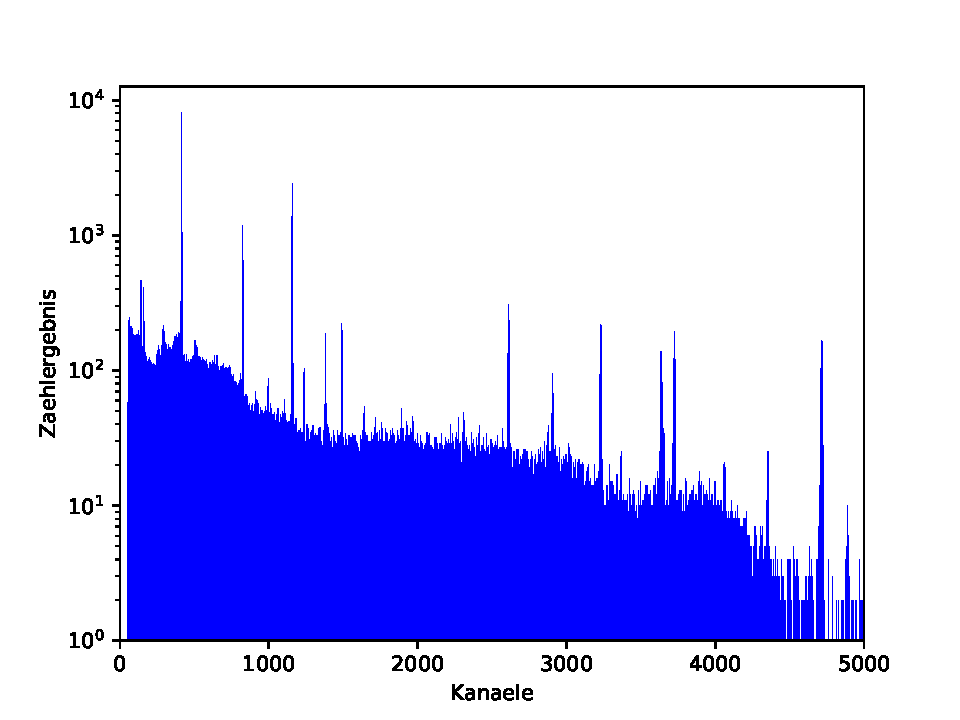
\includegraphics[width=0.8\textwidth]{python/plots/spec1.pdf}
 \caption{Rohdaten der Vermessung des Europium 152 Spektrums.}
 \label{fig:spektrum_eu}
 \end{figure}
Die in Tabelle \ref{tab:atab1} angegebenen Lagen der Spektrallinien werden nach dem in Abschnitt \ref{subsec:a0} beschriebenen Verfahren bestimmt.
\begin{table}
\centering
\caption{Literaturwerte und gemessene Kanäle eines Europium 152 Gammaspektrums \cite{sample}.}
\begin{tabular}{c c c}
\hline \\
Kanal $k$ &Energie $E_\gamma$ in keV & Emissionswahrscheinlichkeit $W$ in \% \\
\hline \\
414.12 & 121.78 & 28.60 \\ 825.86 & 244.70 & 7.60 \\ 997.32 & 295.94 & 0.40 \\ 1158.71 & 344.30 & 26.50 \\ 1382.31 & 411.12 & 2.20 \\ 1491.59 & 443.96 & 3.10 \\ 2273.21 & 678.00 & 2.00 \\ 2310.43 & 688.67 & 0.90 \\ 2612.36 & 778.90 & 12.90 \\ 2908.55 & 867.37 & 4.20 \\ 3231.22 & 964.08 & 14.60 \\ 3368.59 & 1005.30 & 0.60 \\ 3639.40 & 1085.90 & 10.20 \\ 3726.07 & 1112.10 & 13.60 \\ 4353.21 & 1299.10 & 1.60 \\ 4716.58 & 1408.00 & 21.00 \\ 4888.94 & 1457.60 & 0.50 \\
\hline
\end{tabular}
\label{tab:atab1}
\end{table}
In Abbildung \ref{fig:Kalibrierung} werden die entsprechenden Kanäle gegen die Literaturwerte des Eu-Spektrums aufgetragen.
Über eine lineare Ausgleichsrechnung wird die Umrechnungsvorschrift
\begin{align*}
k(E) &= s \cdot E + b \text{, mit}\\
  s &= \SI{3.346+-0.001}{\per\electronvolt}\\
  b &= \SI{ 5.9+-0.8}{}
\end{align*}
zwischen Kanalnummern und Energien in keV bestimmt.
\begin{figure}
\centering
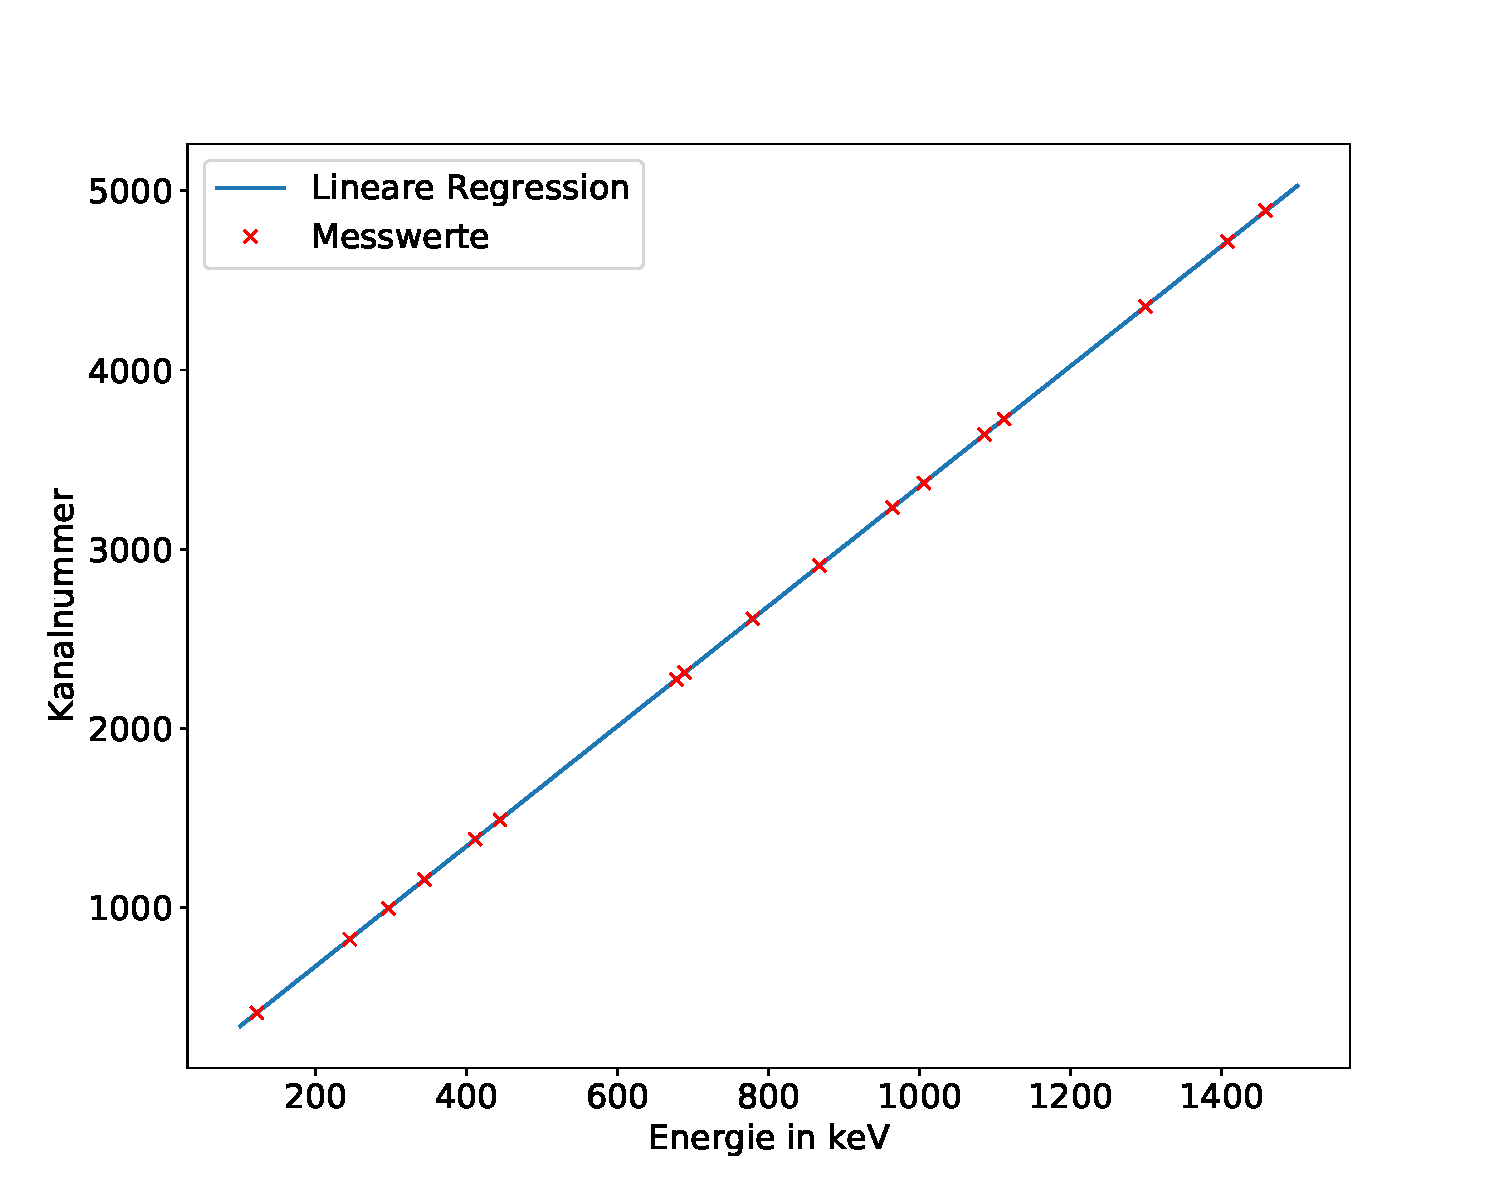
\includegraphics[width=0.8\textwidth]{python/plots/kalibrierung.pdf}
\caption{Lineare Regression der Messwerte aus Tabelle \ref{tab:atab1}}
\label{fig:Kalibrierung}
\end{figure}
Mit Gleichung \eqref{eqn:effizienz} soll die Effizienz der Spektrallinien berechnet werden.
Um die dazu nötige Aktivität des Europiums zum Zeitpunkt der Messung zu bestimmen, wird das exponentielle Zerfallsgesetz
\begin{align}
A_\text{Messung}=A_0\exp\left(\frac{\log(2)}{T_{\frac{1}{2}}}\Delta t\right)
\end{align}
verwendet.
Die Aktivität $A_0$ am 01.10.2000 betrug $\SI{130+-60}{\becquerel}$ und die Halbwertszeit von Europium beträgt $\SI{4943+-5}{\day}$ \cite{sample}.
Das angegebene Datum liefert eine zeitliche Differenz von $\Delta t=\SI{6084}{\day}$, sodass sich eine Aktivität von
\begin{align*}
A_\text{Messung}=\SI{1760+-26}{\becquerel}
\end{align*}
ergibt.
Leider wurde der Abstand $d$ zwischen Probe und Detektor nicht gemessen.
Der Wert von $d=\SI{8.8+-0.3}{\centi\meter}$ wird deshalb dem Protokoll einer befreundeten Gruppe entnommen \cite{abstand}.
Der Radius der Probe beträgt $r=\SI{2.25}{\centi\meter}$ \cite{sample}.
Aus
\begin{align}
\frac{\Omega}{4\pi}=\frac{1}{2}\left( 1- \frac{d}{\sqrt{d^2+r^2}}\right)
\end{align}
lässt sich dann der Raumwinkel $\Omega=\SI{1.96+-0.021}{}$ berechnen.
Mit diesem Wert und den aus den Gauß-Fits berechneten Flächeninhalten der Gauß-Funktionen lassen sich nun die in Tabelle \ref{tab:atab2} angegebenen Effizienzen berechnen.
Dabei ist zu Berücksichtigen, dass die Zählrate aus Formel \ref{eqn:effizienz} gerade den Inhalten geteilt durch die Messdauer $t_\text{Messung}=\SI{7764}{\second}$ entspricht.
\begin{table}
\centering
\caption{Inhalte der Gauß-Fits und die daraus berechneten Effizienzen.}
\begin{tabular}{c c c}
\hline \\
Energie in $\SI{}{\electronvolt}$ & Inhalt & Effizienz in \%\\
\hline \\
121.78 & 28310$\pm$90 & 45.5$\pm$0.6 \\ 244.70 & 4770$\pm$40 & 28.80$\pm$0.5 \\ 295.94 & 230$\pm$30 & 27.0$\pm$3.0 \\ 344.30 & 11700$\pm$70 & 20.3$\pm$0.3 \\ 411.12 & 740$\pm$20 & 15.4$\pm$0.5 \\ 443.96 & 1010$\pm$20 & 15.0$\pm$0.4 \\ 678.00 & 40$\pm$10 & 1.00$\pm$0.3 \\ 688.67 & 240$\pm$20 & 12.0$\pm$1.0 \\ 778.90 & 2320$\pm$40 & 8.3$\pm$0.2 \\ 867.37 & 640$\pm$30 & 7.0$\pm$0.3 \\ 964.08 & 2080$\pm$40 & 6.6$\pm$0.2 \\ 1005.30 & 90$\pm$10 & 7.0$\pm$1.0 \\ 1085.90 & 1170$\pm$40 & 5.3$\pm$0.2 \\ 1112.10 & 1830$\pm$40 & 6.2$\pm$0.2 \\ 1299.10 & 160$\pm$20 & 4.6$\pm$0.5 \\ 1408.00 & 2290$\pm$70 & 5.0$\pm$0.2 \\ 1457.60 & 180$\pm$50 & 16.0$\pm$5.0\\
\hline
\end{tabular}
\label{tab:atab2}
\end{table}
Es wird angenommen, dass die Effizienz $Q$ mit steigender Energie wie eine Potenzfunktion
\begin{align}
Q(E)=c E^{d}
\end{align}
abnimmt.
Die in Abbildung \ref{fig:Effizienz} dargestellte Regressionsrechnung liefert die Parameter
\begin{align*}
c&=\SI{80+-40}{}\\
d&=\SI{-1.03+-0.07}{}\text{ .}
\end{align*}
\begin{figure}
\centering
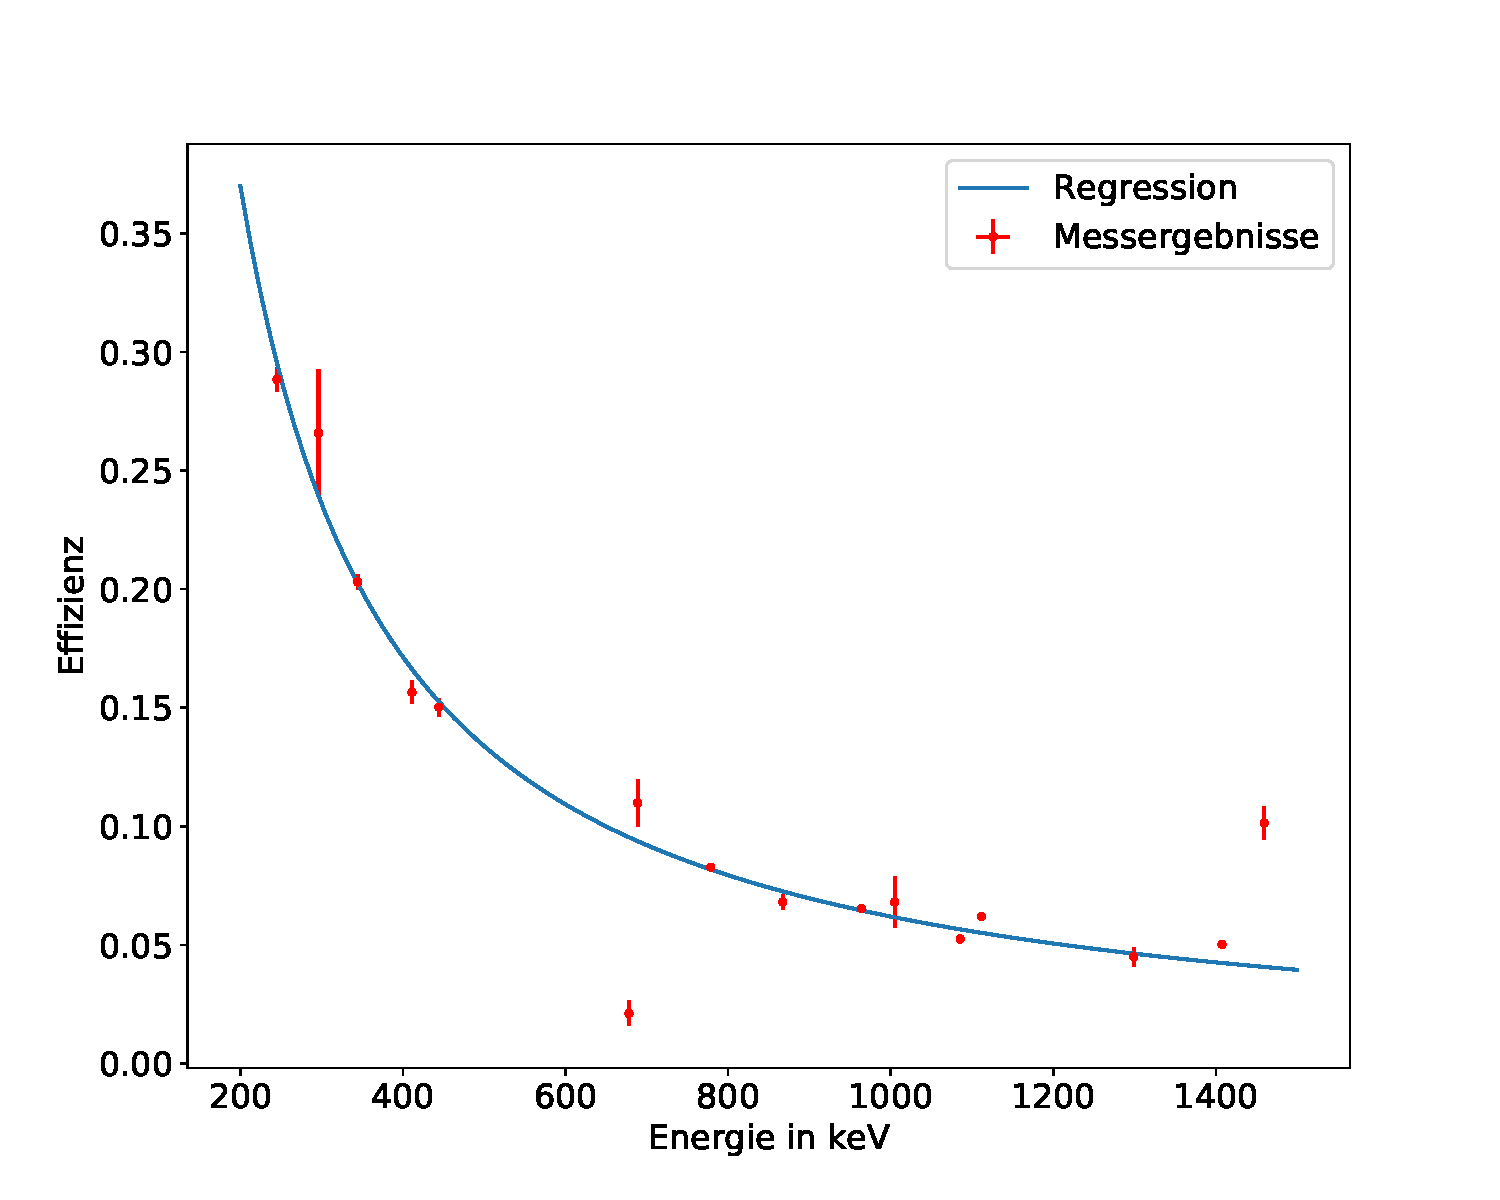
\includegraphics[width=0.8\textwidth]{python/plots/effizienz.pdf}
\caption{Darstellung der Abnahme der Effizienz mit Steigender Energie durch eine Regressionsrechnung. Energien unterhalb von $\SI{150}{\electronvolt}$ werden nicht betrachtet.}
Dabei wird der Peak bei ca. $\SI{778}{\electronvolt}$ vernachlässigt, da eine Inhaltsbestimmung wegen des Untergrunds kaum möglich ist.
\label{fig:Effizienz}
\end{figure}

\subsection{Bestimmungen von Detektoreigenschaften}
\label{subsec:a2}
Um Informationen über Detektoreigenschaften, wie die Energieauflösung, zu gewinnen, wird das Spektrum eines Caesium 137 Strahlers untersucht. Eine graphische Darstellung des aufgenommenen
Spektrums, ist in Abbildung \ref{fig:spectrum_caesium} gegeben.

\subsubsection{Vermessung des Photopeaks}
\label{subsubsec:a21}
Zunächst wird die exakte Position des Phototpeaks(in Kanaelen), mithilfe eines wie in Abschnitt \ref{subsec:a1} beschriebenen Gauss-Fits
möhlichst genau appromiximiert. Es ergeben sich die Fit-Parameter

\begin{align*}
  c_{1} = \SI{1642.409+-17.236}
  c_{2} = \SI{0.058+-0.002}
  c_{3} = \SI{2220.547+-0.036}
  c_{4} = \SI{4.654+-6.670}.
\end{align*}

Der dazugehörige Fit ist in Abbildung \ref{fig:gfit2} zu sehen. Um aus $c_{2}$ die tatsächliche Lage $E$
des Peaks zu bestimmen, wird der in Abscnitt \ref{subsec:a1} gefundene lineare Zusammenhang verwendet.
Es ergibt sich

\begin{align*}
  E_{\text{ph}} = \SI{661.770+-0.011}{\kilo\electronvolt}.
\end{align*}

Weiterhin wird der Inhalt des Peaks bestimmt. Dieser ergibt sich aus Gleichung \eqref{eqn:inhalt}, die allerdings
noch mit der Steigung $a$ des in Abschnitt \ref{subsec:a1} bestimmten linearen Zusammenhangs multipliziert werden muss.
Für den Peak-Inhalt ergibt sich

\begin{align*}
  Z_\text{ph} = \SI{2070+-40}{\kilo\electronvolt}.
\end{align*}
Um ein Maß für die Energieauflösung zu bestimmen, wird nun die Halbwertsbreite, sowie die Zehntelwertsbreite
der Gauss-Funktion bestimmt.
Dazu wird der Zusammenhang

\begin{equation}
  \label{eqn:halbwertsbreite}
  x_{p} = 2 \cdot \sqrt{\frac{\log\left( p^{-1} \right)}{c_{3}}} \cdot a^{-1}
\end{equation}
verwendet. Dabei bezeichnet $a$ die Steigung des in Abschnitt \ref{subsec:a1} bestimmten linearen Zusammenhangs und
$p$ den Anteil an der Peakhöhe auf den die Funktion abgefallen ist.
Es wird jeweils ein Wert von

\begin{align*}
  x_{1/2} = \SI{2.311+-0.032}{\kilo\electronvolt}
\end{align*}

und

\begin{align*}
  x_{1/10} = \SI{4.2+-0.06}{\electronvolt}
\end{align*}
ermittelt.
Der Anteil der Zehntelwertsbreite an der Halbwertsbreite beträgt

\begin{align*}
  \frac{x_{1/10}}{x_{1/2}} = \SI{1.823}.
\end{align*}
Dieser Wert ist charakteristisch für eine Gauss-Funktion, sodass hiermit bestätig wird, dass der Photo-Peak tatsächlich
eine solche Gestalt hat.
Um die Halbwertsbreite vergleichen zu können wird aus der Lage des Photo-Peaks $E_{\text{ph}}$  gemäß

\begin{equation}
    \label{eqn:halbwerttheorie}
    x_{1/2}^{\text{theorie}} \approx 2.35 \cdot \sqrt{\frac{E_\text{ph} \cdot E_{EL}}{10}}
\end{equation}
ein Vergleichswert bestimmt. Die relative Abweichung des über den Fit bestimmten Werts beträgt

\begin{align}
  \frac{\lvert x_{1/2} - x_{1/2}^{\text{th}} \rvert}{x_{1/2}^{\text{th}}} = \SI{29}{\percent}.
\end{align}

\subsubsection{Vermessung des Compton-Kontinuums}
\label{subsubsec:a22}
Zwei charakteristische Positionen im Bereich des Comptonkontinuums sind der Rückstreupeak, sowie die
Comptonkante\footnote{Am Ende des Kontinuums}. Diese werden aus dem in Abbildung \ref{fig:spectrum_caesium} gezeigten
Spektrum abgelesen und in die Energien

\begin{align*}
  x_\text{rueckstreu} &= \SI{188.9+-3.0}{\kilo\electronvolt}\\
  x_\text{comptonkante} &= \SI{465.6+-3.0}{\kilo\electronvolt}
\end{align*}
umgerechnet. Mithilfe von Gleichung \eqref{eqn:rstreupos} lässt sich aus der zuvor bestimmten Energie $E_\text{ph}$
ein Vergleichswert für die Position des Rückstreu-Peaks finden. Gleiches gilt für die Compton-Kante, für die Gleichung
\eqref{eqn:ckante} verwendet wird.
Es ergeben sich die Werte

\begin{align*}
  x_\text{rueckstreu}^\text{theorie} = \SI{184.33+-0.03}{\kilo\electronvolt}\\
  x_\text{comptonkante}^\text{theorie} = \SI{477.44+-0.01}{\kilo\electronvolt}
\end{align*}.
Die relativen Abweichungen betragen jeweils

\begin{align*}
  \frac{\lvert x_\text{rueckstreu} - x_\text{rueckstreu}^\text{theorie} \rvert}{x_\text{rueckstreu}^\text{theorie}} &= \SI{2.5}{\percent}\\
  \frac{\lvert x_\text{comptonkante} - x_\text{comptonkante}^\text{theorie} \rvert}{x_\text{comptonkante}^\text{theorie}} &= \SI{2.5}{\percent}.
\end{align*}

Um den Inhalt des Compton-Kontinuums zu bestimmen, wird für das Intervall von Kanal $800$ bis Kanal $1570$ ein
Fit des Zusammenhangs \eqref{eqn:dsig} durchgeführt. Da sich der Wirkungsquerschnitt proportional zu
der Anzahl an Interaktionen verhalten sollte, wird als Fit-Parameter ein konstanter Vorfaktor $k$ gewählt. Für diesen ergibt
sich

\begin{align*}
  k = \SI{1.089+-0.008 e-8}{}.
\end{align*}
Durch Integration der gefitteten Funktion mit Integrationsgrenzen bei Kanal $55$ und Kanal $1570$, sowie anschließender
Multiplikation mit der Steigung des linearen Zusammenhangs auf Abschnitt \ref{subsec:a1}, ergibt sich für den Inhalt des
Kontinuums

\begin{align*}
  Z_\text{compton-kontinuum} = \SI{11458.8}{\kilo\electronvolt}.
\end{align*}
Dieser Wert kann allerdings nur als grober Richtwert für den tatsächlichen Inhalt des Kontinuums betrachtet werden,
denn die für den Fit verwendeten Daten sind Resultat einer Überlagerung des eigentlichen Compton-Kontinuums mit
Untergrund und Signalen anderer Effekte. Eine graphische Darstellung des Fits ist in Abbildung \ref{fig:kontinuumplot}
zu finden.

\subsubsection{Vergleich von Compton-Kontinuum und Photo-Peak}
\label{subsubsec:a23}
Um die Inhalte des Compton-Kontinuums und des Photo-Peaks zu vergleichen, ist es sinnvoll die jeweilige Absorptionswahrscheinlichkeiten für den Photoeffekt zu
und den Compton-Effekt zu bestimmen. Dafür kann der Zusammenhang \eqref{eqn:wkeit} verwendet werden.
Die Extinktionskoeffizienten werden aus Abbildung \ref{fig:extinktion} grob abgelesen und werden als

\begin{align*}
  \mu_\text{compton} = &\SI{39}{\per\meter}\\
  \mu_\text{photo} = &\SI{0.8}{\per\meter}
\end{align*}
angenommen. \\
Damit ergeben sich die Absorptionswahrscheinlichkeiten

\begin{align*}
  w_\text{compton} &= \SI{78.2}{\percent}\\
  w_\text{photo} &= \SI{3.1}{\percent}
\end{align*}
Das Verhältnis zwischen den Wahrscheinlichkeiten beträgt

\begin{align*}
    \frac{w_\text{compton}}{w_\text{photo}} = 25.4 .
\end{align*}

Dies kann nun mit dem Verhältnis zwischen dem Inhalt des Photopeaks und dem des Compton-Kontinuums verglichen werden.
Diese Verhältnis beträgt

\begin{align*}
  \frac{Z_\text{compton-kontinuum}}{Z_\text{ph}} = 5.5 .
\end{align*}

Dies entspricht einer relativen Abweichung $\delta$ von

\begin{align*}
  \delta = \SI{78.3}{\percent} .
\end{align*}

\FloatBarrier
\begin{figure}
  \centering
  \includegraphics[width=\textwidth]{python/plots/gaussfit}
  \caption{Gaussfit des Photo-Peaks des Caesiumstrahlers.}
  \label{fig:gfit2}
\end{figure}

\begin{figure}
  \centering
  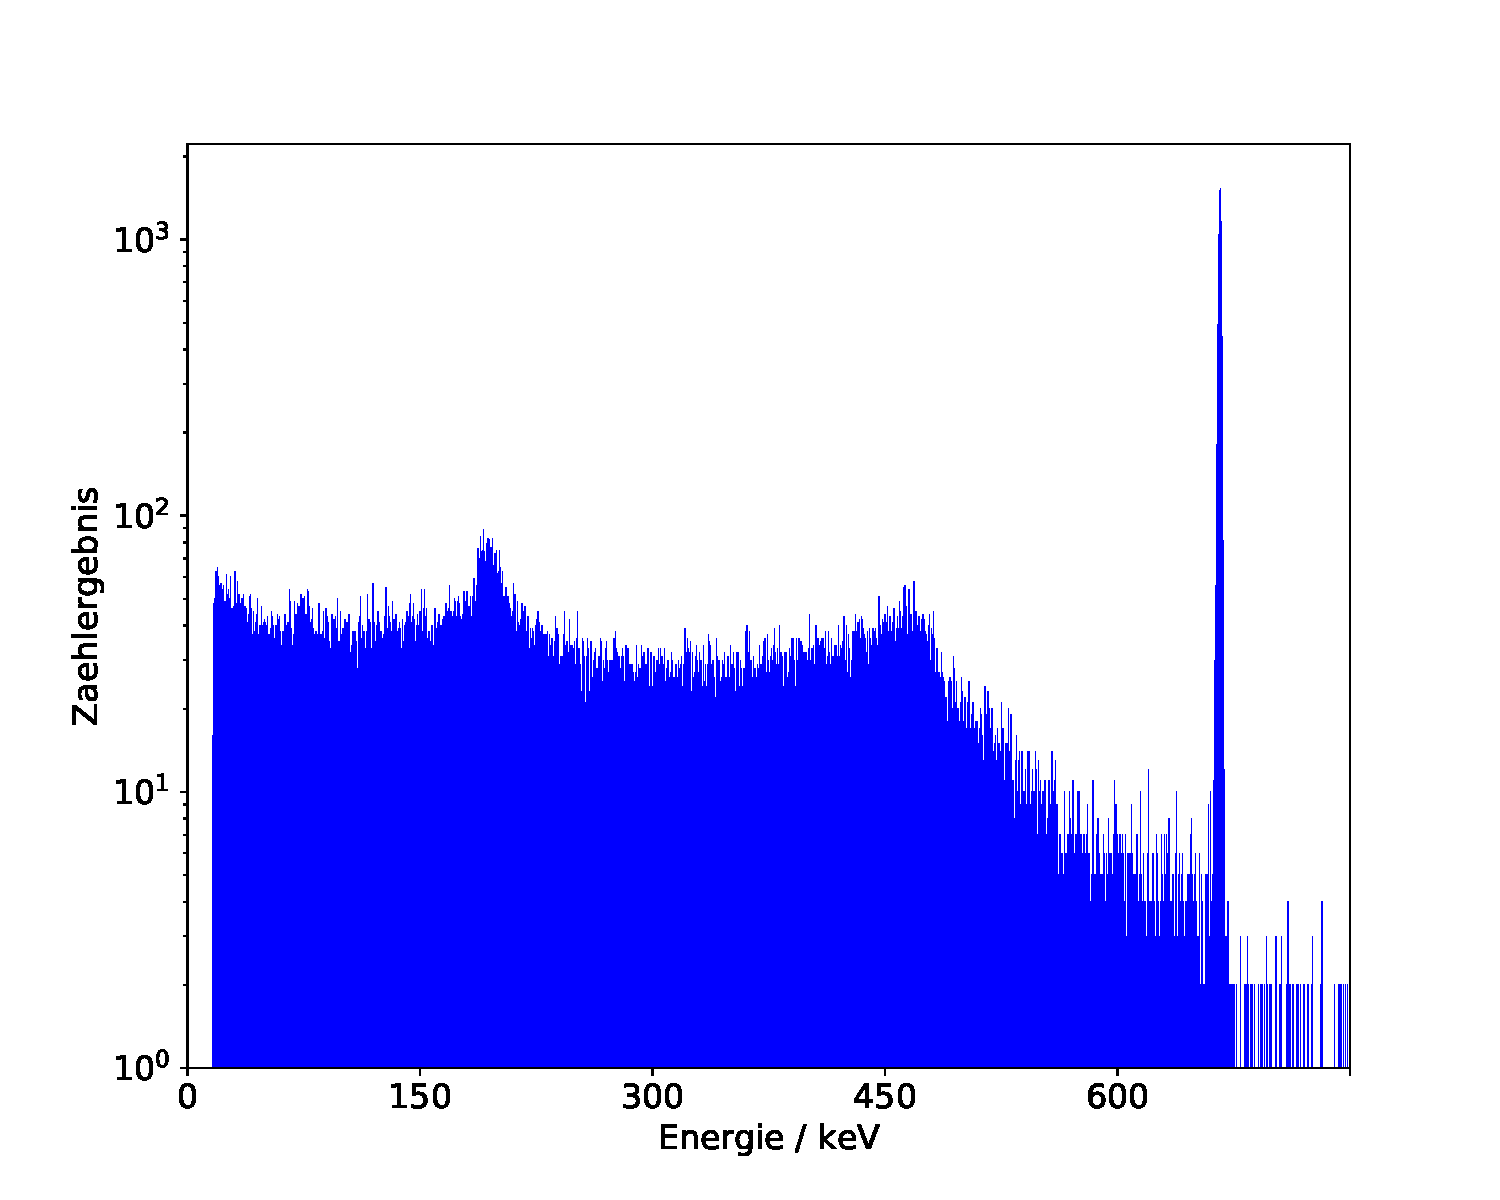
\includegraphics[width=\textwidth]{python/plots/spec2.pdf}
  \caption{Spektrum des Caesium-Strahlers.}
  \label{fig:spectrum_caesium}
\end{figure}

\begin{figure}
  \includegraphics[width=\textwidth]{python/plots/kontinuumfit}
  \caption{Fit zur Bestimmung des Inhalts des Compton-Kontinuums.}
  \label{fig:kontinuumplot}
\end{figure}
\FloatBarrier



\subsection{Aktivitätsbestimmung von Barium 133}
\label{subsec:a3}
In Abbildung \ref{fig:Spektrum_Barium} ist das Spektrum einer Barium 133 Probe dargestellt.
\begin{figure}
\centering
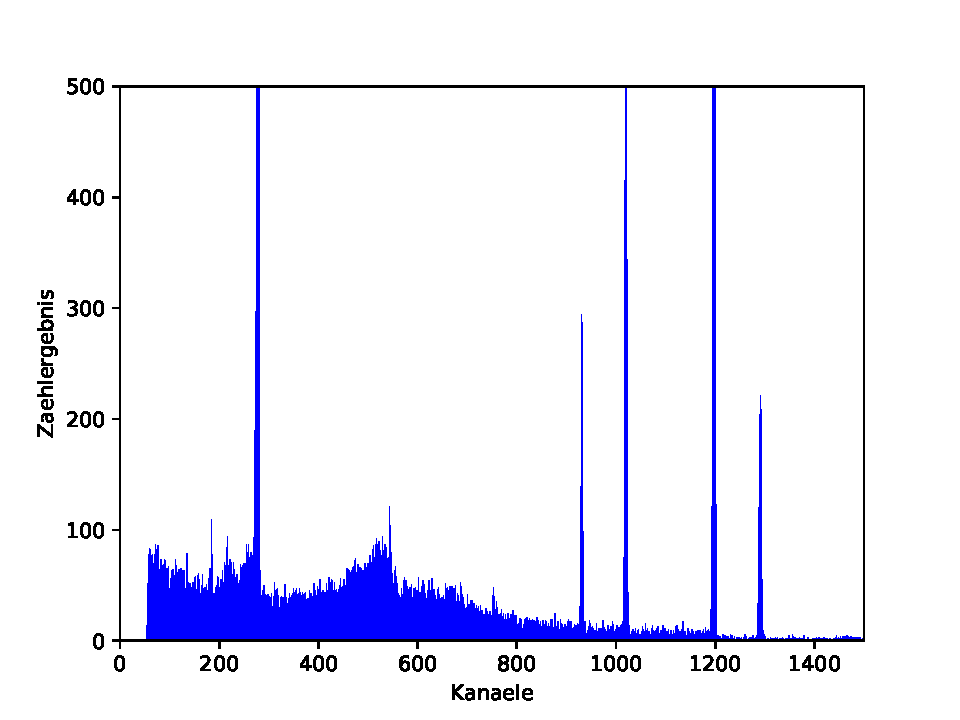
\includegraphics[width=0.8\textwidth]{python/plots/spec3.pdf}
\caption{Gamma-Spektrum einer Barium 133 Probe.}
\label{fig:Spektrum_Barium}
\end{figure}
Um die Aktivität der Probe zum Zeitpunkt der Messung zu bestimmen wird Gleichung (\ref{eqn:effizienz}) verwendet.
Wie in Abschnitt \ref{subsec:a0} beschrieben wird die Lage und der Inhalt der verschiedenen Peaks berechnet.
Mit der in Abschnitt \ref{subsec:a1} bestimmten Beziehung $Q(E)$ zwischen Effizienz und Energie, dem bekannten Raumwinkel $\Omega$ und den in Tabelle \ref{tab:a_d_1} angegebenen Emissionswahrscheinlichkeiten wird von jeder Spektrallinie einzeln auf die Aktivität der Probe geschlossen.
Die Ergebnisse dieser Rechnung finden sich ebenfalls in Tabelle \ref{tab:a_d_1}.
\begin{table}
\centering
\caption{Für die Berechnung der Aktivität wichtige Daten je Spektrallinie \cite{sample}.}
\begin{tabular}{c c c c}
\hline \\
Lage in keV & Intensität in s$^{-1}$&  Emissionswahrscheinlichkeit in \%& Aktivität in $\SI{}{\becquerel}$\\
\hline \\
184.93 $\pm$0.15  &  0.04  $\pm$0.02  &  2.20  &  102  $\pm$57 \\ 278.34 $\pm$0.02  &  2.93  $\pm$1.59  &  34.06  &  540  $\pm$293 \\ 543.81 $\pm$0.32  &  0.14  $\pm$0.10  &  0.65  &  1365  $\pm$919 \\ 753.17 $\pm$0.15  &  0.08  $\pm$0.05  &  0.45  &  1101  $\pm$678 \\ 931.69 $\pm$0.02  &  1.54  $\pm$0.92  &  7.20  &  1341  $\pm$804 \\ 1020.80 $\pm$0.03  &  3.96  $\pm$2.40  &  18.30  &  1360  $\pm$822 \\ 1198.10 $\pm$0.01  &  13.29  $\pm$8.14  &  62.10  &  1344  $\pm$823 \\ 1291.30 $\pm$0.05  &  1.96  $\pm$1.21  &  8.90  &  1382  $\pm$853 \\
\hline
\end{tabular}
\label{tab:a_d_1}
\end{table}
Als Mittelwert dieser einzelnen Aktivitäten ergibt sich das gesamt Ergebnis der Aktivität
\begin{align*}
A_{Ba-133}=\SI{1320+-100}{\becquerel} \text{ .}
\end{align*}
Die Aktivitäten, welche aus den ersten beiden Spektrallinien berechnet werden, werden bei dieser Rechnung vernachlässigt.


\subsection{Untersuchung von Zerfallsketten in einem unbekannten Strahler }
\label{subsec:a4}
Es wird eine raioaktive Probe untersucht, deren Spektrum in Abbildung \ref{fig:spectrum_4} zu sehen ist.
Zu untersuchen ist, welche radioaktiven Nuklide enthalten sind. Dazu werden die identzifizierbaren Spektrallinien
mit denen der in der Versuchsanleitung \cite{sample} angegebenen Zerfallsreihen verglichen.  Die Position
der Spektrallinien werden, wie schon in den vorausgegangenen Abschnitten \ref{subsec:a1} und \ref{subsec:a2}, zunächst
grob aus dem aufgenommenen Spektrum abgelesen und dann genauer mithilfe eines Gauss-Fits lokalisiert.
Es ergeben sich die in Tabelle \ref{tab:spektrallinien_4}  angegebenen Spektrallinien. Es lässt sich erkennen, dass
Teile der Uran 238 Zerfallsreihe auftreten. Dabei lässt sich der Teil an dem Thorium 234, Paladium 234, Radium 226,
Blei 214 und Bismuth 214 beteiligt sind, gut identifizieren. Die jeweils nicht gefundenen Linien der genannten Nuklide
treten meist mit einer niedrigen Wahrscheinlichkeit auf und oder liegen bei sehr kleinen Energien. Eine Ausnahme bildet
Paladium 234. \\
In Tabelle \ref{tab:nuklide} sind die Spekrallinien der jeweiligen Nuklide aufgelistet.

\FloatBarrier
\begin{table}
  \centering
  \caption{Tabelle der in Spektrum 4 gefundenen Spektrallinien.}
  \label{tab:spektrallinien_4}
  \begin{tabular}{c c c}
    \toprule
    $\text{Kanal }$ & $E \text{ in } \si{\kilo\electronvolt}$ & $ \text{passendes Nuklid} $\\
    \midrule
    \SI{4716.53+-0.38} & \SI{1407.62+-0.11} & Bi 214 \\
    \SI{4615.05+-0.28} & \SI{1377.30+-0.08} & Bi 214\\
    \SI{4291.63+-0.43} & \SI{1280.65+-0.13} &  \\
    \SI{4148.37+-0.19} & \SI{1237.84+-0.06} & \\
    \SI{3753.91+-0.13} & \SI{1119.97+-0.04} & Bi 214\\
    \SI{3355.26+-0.81} & \SI{1000.85+-0.24} &  \\
    \SI{3130.60+-0.24} & \SI{933.71+-0.07} & Bi 214 \\
    \SI{2812.84+-0.48} & \SI{838.76+-0.14} & \\
    \SI{2703.29+-0.56} & \SI{806.02+-0.17} &  \\
    \SI{2635.46+-0.34} & \SI{785.76+-0.10} & Bi 212\\
    \SI{2576.44+-0.15} & \SI{768.12+-0.04} & Bi 214 \\
    \SI{2232.49+-0.20} & \SI{665.34+-0.06} &  \\
    \SI{2044.51+-0.03} & \SI{609.17+-0.01} & Bi 214 \\
    \SI{1183.75+-0.01} & \SI{351.95+-0.00} & Pb 214 \\
    \SI{994.27+-0.01} & \SI{295.33+-0.00} & Pb 214 \\
    \SI{816.14+-0.03} & \SI{242.10+-0.01} & Pb 214\\
    \SI{628.91+-0.03} & \SI{186.16+-0.01} & Ra 226\\
    \SI{335.03+-1.77} & \SI{98.34+-0.53} Pa 234& \\
    \SI{317.00+-0.62} & \SI{92.95+-0.19} & Th 234\\
    \SI{264.46+-0.05} & \SI{77.25+-0.01} & \\
    \bottomrule
  \end{tabular}
\end{table}

\begin{table}
  \centering
  \caption{Spektrallinien der identifizierten Nuklide(Informationen aus Versuchsanleitung).\cite{sample}}
  \label{tab:nuklide}
  \begin{tabular}{c c c c}
    \toprule
    $\text{\text{Nuklid}}$ & $E \text{ in } \si{\kilo\electronvolt}$ & $ \text{Wahrscheinlichkeit} $ & $\text{identifiziert (j/n)}$\\
    \midrule
    Th 234 & \SI{63}{} & \SI{3.5}{\percent} & \text{n} \\
           & \SI{93}{} & \SI{4}{\percent} & \text{j} \\
    Pa 234 & \SI{100}{} & \SI{50}{\percent} & \text{j} \\
           & \SI{126}{} & \SI{26}{\percent} & \text{n} \\
           & \SI{220}{} & \SI{14}{\percent} & \text{n} \\
           & \SI{360}{} & \SI{13}{\percent} & \text{n} \\
           & \SI{560}{} & \SI{15}{\percent} & \text{n} \\
           & \SI{700}{} & \SI{24}{\percent} & \text{n} \\
           & \SI{900}{} & \SI{70}{\percent} & \text{n} \\
           & \SI{1080}{} & \SI{12}{\percent} & \text{n} \\
    Ra 226 & \SI{186}{} & \SI{4}{\percent} & \text{j} \\
    Pb 214 & \SI{53}{} & \SI{1}{\percent} & \text{n} \\
           & \SI{242}{} & \SI{4}{\percent} & \text{j} \\
           & \SI{296}{} & \SI{19}{\percent} & \text{j} \\
           & \SI{352}{} & \SI{36}{\percent} & \text{j} \\
    Bi 214 & \SI{609}{} & \SI{47}{\percent} & \text{j} \\
           & \SI{769}{} & \SI{5}{\percent} & \text{j} \\
           & \SI{935}{} & \SI{3}{\percent} & \text{j} \\
           & \SI{1120}{} & \SI{17}{\percent} & \text{j} \\
           & \SI{1378}{} & \SI{5}{\percent} & \text{j} \\
           & \SI{1400}{} & \SI{4}{\percent} & \text{j} \\
           & \SI{1509}{} & \SI{2}{\percent} & \text{n} \\
           & \SI{1728}{} & \SI{3}{\percent} & \text{n} \\
           & \SI{1764}{} & \SI{17}{\percent} & \text{n} \\
           & \SI{2204}{} & \SI{5}{\percent} & \text{n} \\
     \bottomrule
  \end{tabular}
\end{table}
\FloatBarrier

\begin{figure}
  \centering
  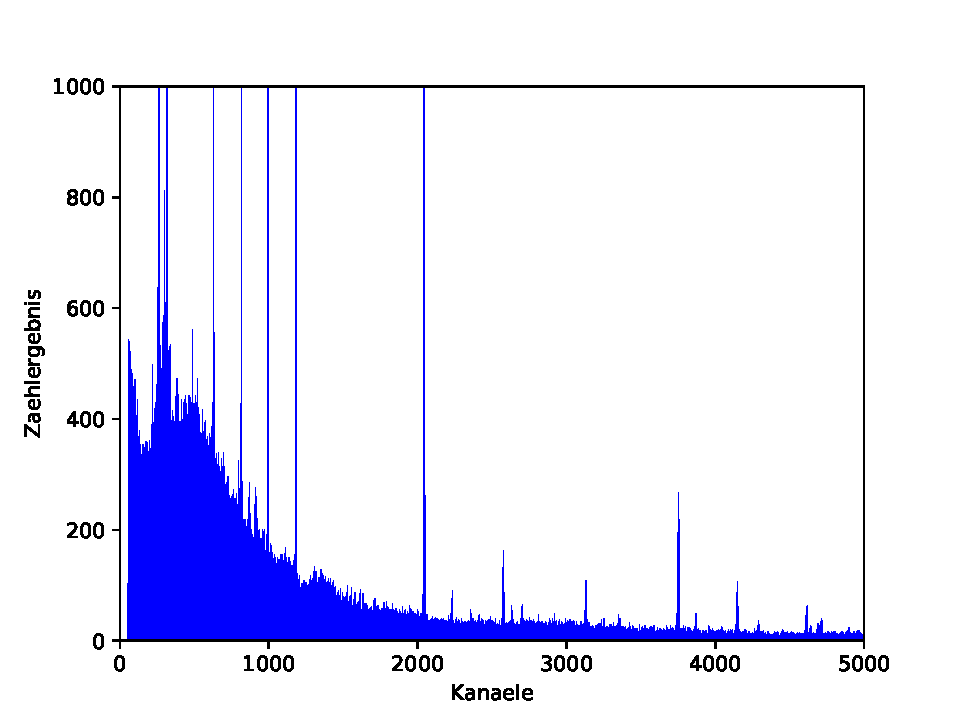
\includegraphics[width=\textwidth]{python/plots/spec4}
  \caption{Spektrum des Unbekannten Strahlers.}
  \label{fig:spectrum_4}
\end{figure}



%\begin{figure}
%  \centering
%  \includegraphics{plot.pdf}
%  \caption{Plot.}
%  \label{fig:plot}
%\end{figure}
